Determining the high-level control-flow structure from a RTL description
of a circuit would be difficult both automatically and manually.
Extracting from a high level input source manually is easier but it would
be challenging for larger designs, however it can be easily automated by
transforming the input into a control and data flow graph (CDFG).
StitchUp can automatically perform this extraction as a compiler flag
for the LegUp HLS tool.

\begin{figure}[h]
\centering
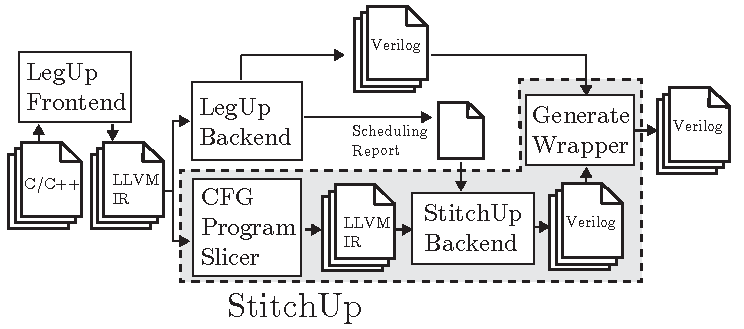
\includegraphics[width=3.5in]{./imgs/tool-flow.pdf}
\caption{Tool Flow Overview diagram}
\label{fig:tool_flow_diagram}
\end{figure}

LegUp is an open source HLS tool built upon LLVM intermediate representation (LLVM-IR) which has
a similar level of abstraction to assembly code.
LLVM-IR has two important features for writing compiler optimisations:
firstly all instructions are in single static assignment form (SSA) where every variable is only
assigned once; and secondly instructions are grouped into straight-line sequences known as basic blocks (BB)
where there is only one entry branch at the very start of the block, and one exit branch at the very end.

Figure \ref{fig:tool_flow_diagram} shows the transformation of an input C program
to a Control-flow protected
Verilog circuit description, with StitchUp sections highlighted in grey.
Initially the C input is passed into the LegUp frontend which is
a series of LLVM passes that
perform various tasks such as annotating instructions with pipelining information.
This outputs an LLVM-IR represnetation which is passed both into the backend of LegUp,
to generate the
original unprotected circuit, and into the frontend of StitchUp to generate a circuit
consisting of just the control-flow structure.
Finally a wrapper script connects the original circuit to the duplicate control-flow circuit
along with comparison logic to ensure that the state registers match.

\begin{figure}[h]
\centering
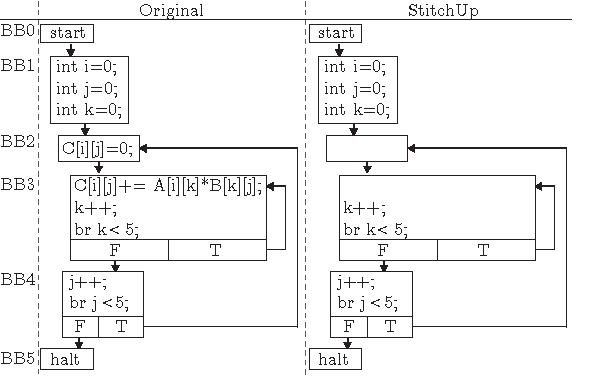
\includegraphics[width=3.5in]{./imgs/mmm_cdfg.pdf}
\caption{Control-Data-Flow Diagram for Matrix Multiplication example}
\label{fig:mmm_cdfg}
\end{figure}

\subsection{Extracting the Control Structure Instruction Set}
The LLVM-IR which is passed into the frontend of StitchUp is naturally arranged
into a Control and Dataflow graph (CDFG) format,
where each node of the graph is a basic block and edges are branches between them.
An example of the CDFG for the matrix multiplication in listing \ref{lst:MMM}
is shown on the left side of Figure \ref{fig:mmm_cdfg}.

The aim of the StitchUp frontend is to extract all SSA instructions that influence
any branch decisions within this CDFG and generate LLVM-IR containing just these
instructions but with the same structure.
To achieve this a control structure instruction set (CSIS) is generated for every basic
block of the input program.

For a basic block, $B$, $CSIS_{B}$ is a set of all SSA instructions in $B$ and
all successors of $B$ that may effect future branch decisions.
Every $CSIS_{B}$ is a complete program and creating a circuit from it would
enable the protection of every control-flow decision from $B$ onwards in the
original programs execution.
If we want to protect the control-flow structure for the entire circuit then
we need to use $CSIS_{E}$, where $E$ is the first basic block in the input program
to generate the error detection hardware.

To calculate every $CSIS$ a fixed point algorithm is used iterating over the CDFG
in a backwards fashion until the $CSIS$ for each basic block is stable.
In each iteration the $CSIS_{i}$ for basic block $i$ is
updated using the following rules:
\begin{enumerate}
    \item For all successor nodes, $j$, of $i$ add every element of $CSIS_j$ to $CSIS_i$.
    \item All branch instructions and operands are added to $CSIS_i$
    \item Any instruction within $i$ that is used as an operand by an element of $CSIS_i$ is added to $CSIS_i$
\end{enumerate}

Figure \ref{fig:mmm_cdfg} on the left shows the CDFG for the original matrix
multiplication function in Listing \ref{lst:MMM}, while the right shows
the control structure shadow version constructed from $CSIS_{BB0}$ where the
inner dot product floating point operations have been discarded.
Using this example we can step through demonstrating the $CSIS$ construction:
\begin{itemize}
\item initially start at $BB4$ attempting to build $CSIS_{BB4}$:
since $BB4$ has no successor nodes the first step is skipped, however for the second step the \lstinline{return}
instruction is added to $CSIS_{BB4}$, and the third step is skipped since no other instructions exist.

\item Moving backwards to $BB3$ the first step adds every element of $CSIS_{BB4}$ to $CSIS_{BB3}$ to give 
$CSIS_{BB3}=$ \{\lstinline{return}\}, then since $CSIS_{BB1}$ is currently empty nothing is added from here; the second step then adds the conditional branch and it's operand
instruction to the current set to give $CSIS_{BB3}= $\{\lstinline{return}, \lstinline{br j<5}\} ;
finally for step 3 \lstinline{j} is used in a member of $CSIS_{BB3}$ in \lstinline{br j<5} so the instruction
\lstinline{j++} is added to $CSIS_{BB3}$. This means that at this point $CSIS_{BB3} =$
\{\lstinline{return},\lstinline{br j<5}, \lstinline{j++}\}

\item For $BB2$ in the first step we take all the elements from the successor node $BB3$, and ignore the fact
that it has itself as a successor, so that we get $CSIS_{BB2} =$ \{\lstinline{return},\lstinline{br j<5}, \lstinline{j++}\}.
Then just like before we can add the branch instruction, \lstinline{br k<5}, using rule 2 and the incrementor for the branch
conditional variable \lstinline{k} using rule 3. 
The instruction \lstinline{C[i][j] += A[i][k]*B[k][j]} is not added to $CSIS_{BB2}$ since no instruction
within $CSIS_{BB2}$ depends on it. This leaves 

\end{itemize}

The analysis will continue in this fashion looping over all the Basic Blocks until a fixed
point on every $CSIS$ is obtained.
Once this has been completed it then uses the topmost $CSIS$, in this case $CSIS_{BB0}$ to
generate an LLVM-IR program containing only the control structure of the original
source.

The output of the StitchUp frontend along with the scheduling report from LegUp
implementation of the original circuit are passed into the StitchUp backend, which identical
to the LegUp Backend with a few modifications to the FSM generation.
LegUp schedules operations in such a way that if an instruction requires more than a single
clock cycles to execute then an FSM state is created for each clock cycle.
This means that if instructions are removed via the StitchUp analysis then potentially
the FSM for the StitchUp circuit could be generated missing these extra scheduling states.
For this reason the scheduling report is used to detect instances of where this situation has occurred,
and include these lost states into the StitchUp FSM.


Finally the wrapper scripts take the original LegUp circuit and the StitchUp circuit and
connect them together.
To do this the scripts expose the FSM state registers for each of the circuits and
generate logic to inspect them every clock cycle.
AXI interfaces are also generated, so that the circuits can be easily tested on Xilinx Zynq devices.
